\section{Projection onto the plane of the sky}
\label{sec:projection}

In this section we calculate the apparent shape on the plane of the
sky of the limb brightened border of a shock or shell that is
idealized as as arbitrary cylindrically symmetric surface.

%Note: I'm aware that some of this material should be moved to an appendix, but I think it will be a future edition.
\subsection{Frames of reference}


Consider body-frame cartesian coordinates $(x,y,z)$, where \(x\) is
the symmetry axis, and spherical polar coordinates
\((R, \theta, \phi)\), where \(\theta\) is the polar angle and
\(\phi\) the azimuthal angle.  Since the surface is cylindrically
symmetric, it is can be specified as $R = R(\theta)$, so that
cartesian coordinates on the surface are:
\begin{equation}
\left(\begin{array}{c}
x \\ y \\ z
\end{array}
\right) = R(\theta)\left(\begin{array}{c}
\cos\theta \\
\sin\theta\cos\phi \\
\sin\theta\sin\phi
\end{array}\right).
\end{equation} 
Suppose that the viewing direction makes an angle \(i\) with the \(z\)
axis, so that we can define observer-frame coordinates
\((x', y', z')\), which are given by the rotating the body-frame
coordinates:
\begin{equation}
\left(\begin{array}{c}
x' \\ y' \\ z'
\end{array}
\right) = \left(\begin{array}{c}
x\cos i - z\sin i\\
y \\
z\cos i + x\sin i
\end{array}\right).
\label{eq:Trans}
\end{equation} 
The relationship between the two frames is illustrated in
Figure~\ref{fig:projection-pos}.  All quantities in the observer's
frame are denoted by attaching a prime to the equivalent quantity in
the body frame.  The celestial coordinates on the ``plane of the sky''
are given by \((x', y')\) with \(x'\) being the projected symmetry
axis of the surface, while the line of sight lies along \(-z'\).  The
inclination angle \(i\) is defined so that \(i = 0^\circ\) when the
surface is viewed perpendicular to its axis (\textit{side on}) and
\(i = 90^\circ\) when it is viewed along its axis (\textit{end on}).

\begin{figure}
  \centering
  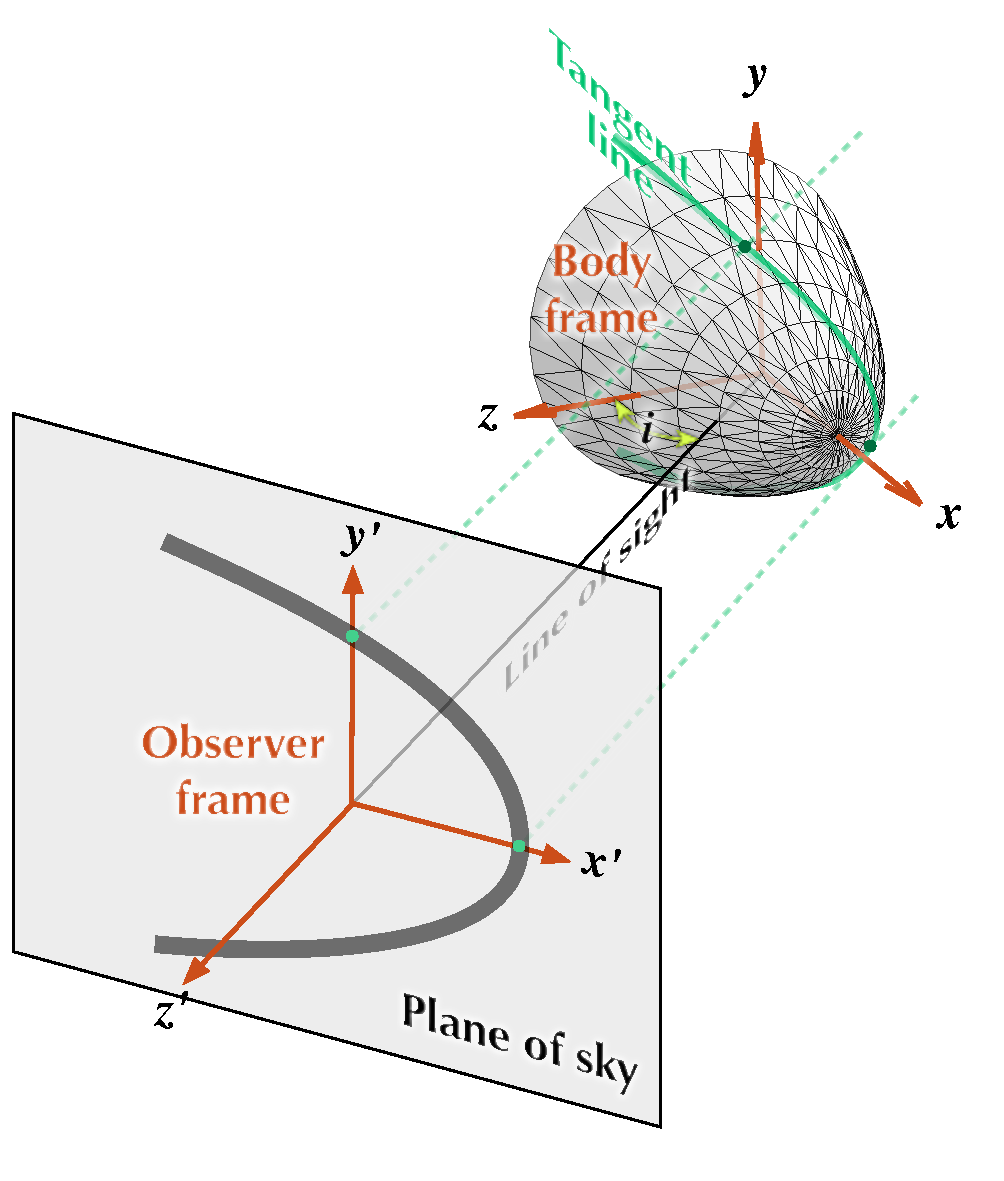
\includegraphics[width=\linewidth]{figs/projection-pos}
  \caption{Relationship between body frame (unprimed coordinates) and
    observer frame (primed coordinates).}
  \label{fig:projection-pos}
\end{figure}

\subsection{Tangent line}

The normal and tangent vectors to the shell's border in the shell's frame are given by:
\begin{align}
\hat{t} = \left(\begin{array}{c}
-\cos\alpha \\
\sin\alpha\cos\phi\\
\sin\alpha\sin\phi
\end{array}\right)\\
\hat{n} = \left(\begin{array}{c}
\sin\alpha \\
\cos\alpha\cos\phi \\
\cos\alpha\sin\phi
\end{array}\right)
\end{align}
Where:
\begin{align}
\tan\alpha = -\left.\frac{dy}{dx}\right|_{R(\theta)} \\
\label{eq:tanalpha}
\end{align}
Then we apply the transformation (\ref{eq:Trans}) to the normal and tangent vectors to obtain:
\begin{align}
\hat{n}' &= \left(\begin{array}{c}
(\cos\theta+\omega\sin\theta)\cos i -(\sin\theta-\omega\cos\theta)\sin i \sin\phi\\
(\sin\theta-\omega\cos\theta)\cos\phi \\
(\cos\theta+\omega\sin\theta)\sin i + (\sin\theta-\omega\cos\theta)\sin\phi\cos i
\end{array}\right)\\
\hat{t}' &= \left(\begin{array}{c}
-(\sin\theta-\omega\cos\theta)\cos i - (\cos\theta+\omega\sin\theta)\sin\phi\sin i \\
(\cos\theta+\omega\sin\theta)\cos\phi \\
-(\cos\theta+\omega\sin\theta)\sin i + (\sin\theta-\omega\cos\theta)\sin\phi\cos i
\end{array}\right)
\end{align}
Where $\omega = \frac{1}{R}\frac{dR}{d\theta}$

In the thin shell case, the limb brightened border of the shell is such that $\hat{n}'\cdot \hat{z}'$. 
The values for $\phi$ that satisfy this relation for each inclination $i$ are given by:
\begin{equation}
\sin\phi_t = \tan i\tan\alpha = \tan i \frac{1+\omega\tan\theta}{\omega-\tan\theta}
\label{eq:tanphi}
\end{equation}
With this, the coordinates of the limb brightened shell are given by:
\begin{equation}
\left(\begin{array}{c}
x'_t \\ y'_t \\ z'_t
\end{array}\right)= R(\theta)\left(\begin{array}{c}
\cos\theta\cos i - \sin\theta\sin\phi_t \sin i \\
\sin\theta(1-\sin^2\phi_t)^{1/2} \\
\cos\theta\sin i +\sin\theta\sin\phi_t\cos i
\end{array}\right)
\label{eq:tangential}
\end{equation} 

It is important to note that the equation (\ref{eq:tanphi}) does not have a solution for arbitrary values for $\theta$ and $i$, since
it's required that $|\sin\phi_t|<1$. If $i\neq 0$, then, the  allowed values for $\theta$ are such that $\theta > \theta_\parallel$, where
$\theta_\parallel$ is given implicitly by:
\begin{align}
\tan\theta_\parallel = \frac{|\tan i| + \omega(\theta_\parallel)}{1-\omega(\theta_\parallel) |\tan i|}
\label{eq:thetapar}
\end{align}

\subsection{Parallel and perpendicular projected shell radii}

Considering further applications to bow shocks, we will consider open shells. In order to compare the shell shape given by $R(\theta)$ with observations,
it is convenient to define the following apparent radii in the observer frame: $R'_\parallel$ and $R'_\perp$. These are projected distances of the shell tangent line
from the origin. The first is measured in the direction of the symetry axis, and the second in a perpendicular direction. More concretely $R'_\parallel = x'_t(y'_t=0)$
and $R'_\perp = y'_t(x'_t=0)$. From equations (\ref{eq:tanphi}) and (\ref{eq:tangential}) we find that:
\begin{align}
R'_\parallel = R(\theta_\parallel)\cos(\theta + i) \label{eq:Rpar} 
\end{align}
Where $\theta_\parallel$ is the solution of equation (\ref{eq:thetapar}), and
\begin{align}
R'_\perp = R(\theta_\perp)\sin\theta_\perp\left(1-\sin^2(\phi_t(\theta_\perp))\right)^{1/2}
\end{align}
Where $\theta_\perp$ is the solution of the next implicit equation:
\begin{align}
\cot\theta_\perp = \frac{1-\left(1+\omega(\theta_\perp)^2\sin^22i\right)^{1/2}}{2\omega(\theta_\perp\cos^2 i)}
\end{align}


%%% Local Variables:
%%% mode: latex
%%% TeX-master: "proplyd-bowshocks"
%%% End:

